\chapter{Synthetic validation and executed diagnostics}
\label{ch:synthetic}\label{sec:experiments}
\chapterpromise{Real recovery, calibration, portability, approximation, and scaling outputs interpreted at the exact scope supported by their archived protocols.}

\subsection{Single-sequence Gaussian illustration}
\label{sec:single_synth}

We begin with a Gaussian sequence containing two true changepoints. Figure~\ref{fig:single_synth}
shows two complementary outputs: the marginal posterior probability that each interior index is a
boundary, and the exported joint MAP segmentation together with segment-level posterior intervals.
The two dominant posterior spikes align with the true changepoints, while a smaller shoulder of
posterior mass just before the first jump reflects local ambiguity caused by a short transitional
run of noisy observations. That ambiguity is visible again in the bottom panel, where the exported
fit inserts a short intermediate segment before settling into the large middle plateau.

\begin{figure}[H]
    \centering
    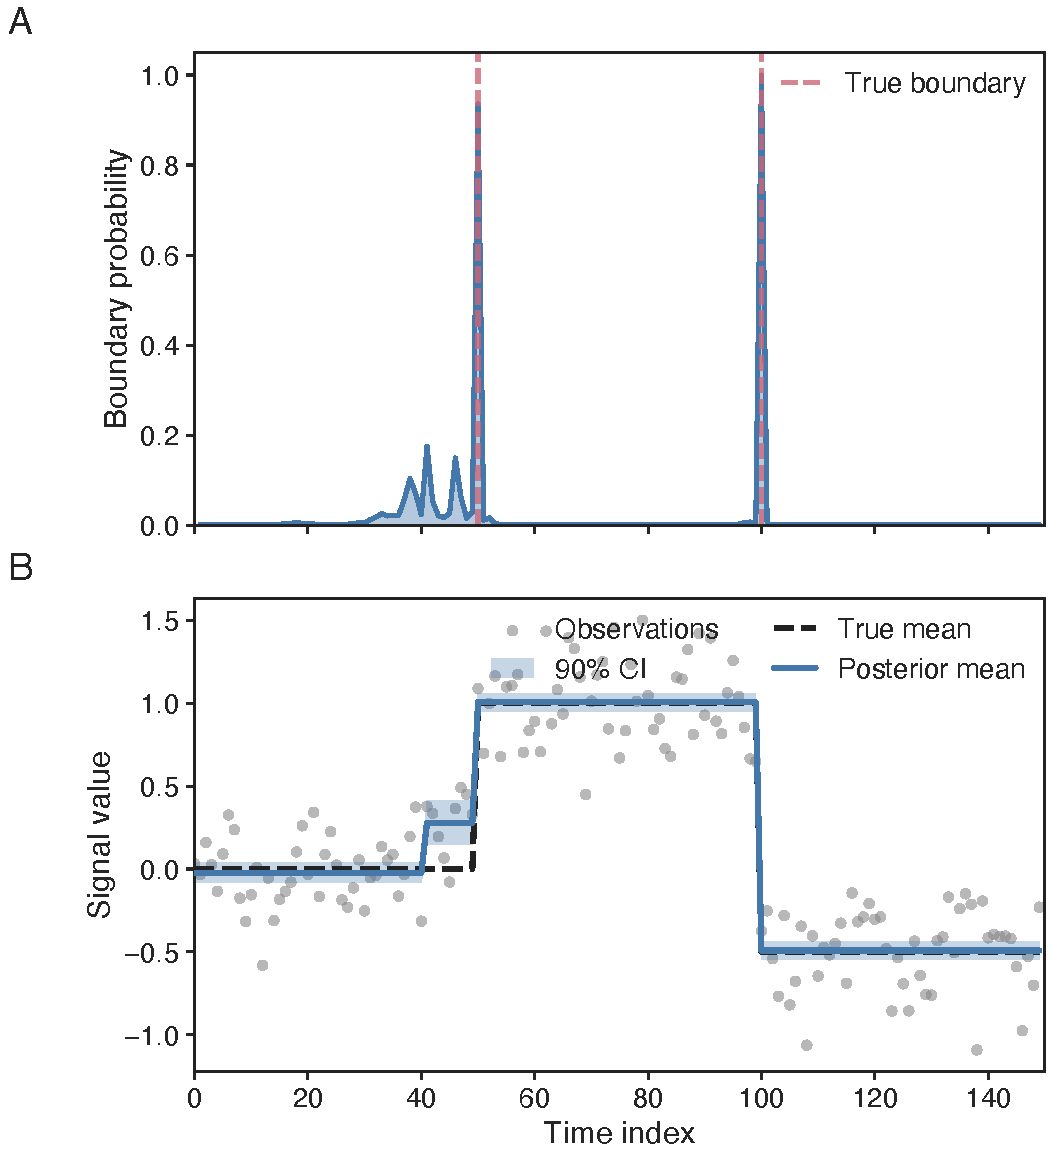
\includegraphics[width=\textwidth]{shared/figures/results/fig1_synthetic_gaussian.pdf}
    \caption{Single-sequence Gaussian example. Top: marginal posterior probability that each interior index $i\in\{1,\dots,n-1\}$ is a changepoint, with dashed vertical lines marking the true changepoints. Bottom: observed data, true latent mean, exported joint MAP segmentation, and 90\% segment-level posterior intervals.}
    \label{fig:single_synth}
\end{figure}

\begin{table}[H]
    \centering
    \begin{tabular}{lr}\toprule
Quantity & Value\\\midrule
Selected $k$ (\texttt{k\_ml\_}) & 4\\
Posterior mean $\mathbb{E}[k]$ & 4.742\\
MAP $k$ & 4\\
$\log p(y)$ & -18.031\\
\bottomrule\end{tabular}

    \caption{Posterior summary for the single-sequence Gaussian example in Figure~\ref{fig:single_synth}. The table separates the displayed exported segmentation from posterior summaries of the segment count.}
    \label{tab:posterior_summary}
\end{table}

Table~\ref{tab:posterior_summary} makes an important methodological point explicit: the displayed
segmentation and the posterior over the segment count are related but not identical objects. In the
archived example, the exported joint MAP segmentation uses four segments, while the posterior mean
$\mathbb{E}[k\mid y]$ is larger, indicating residual posterior mass on more highly segmented
configurations. This is precisely why the book distinguishes sum-product posterior summaries from
max-sum exported segmentations.

\subsection{Likelihood-family showcase}

BayesBreak is designed so that the global DP layer does not depend on the observation model once
block evidences are available. Figure~\ref{fig:family_showcase} visualizes this portability across
three conjugate families (Gaussian, Poisson, Binomial) and one low-dimensional quadrature example
for $(0,1)$-valued responses. Across all four panels, the fitted piecewise-constant signal tracks
the true latent parameter closely and preserves the correct qualitative segmentation pattern.

\begin{figure}[H]
    \centering
    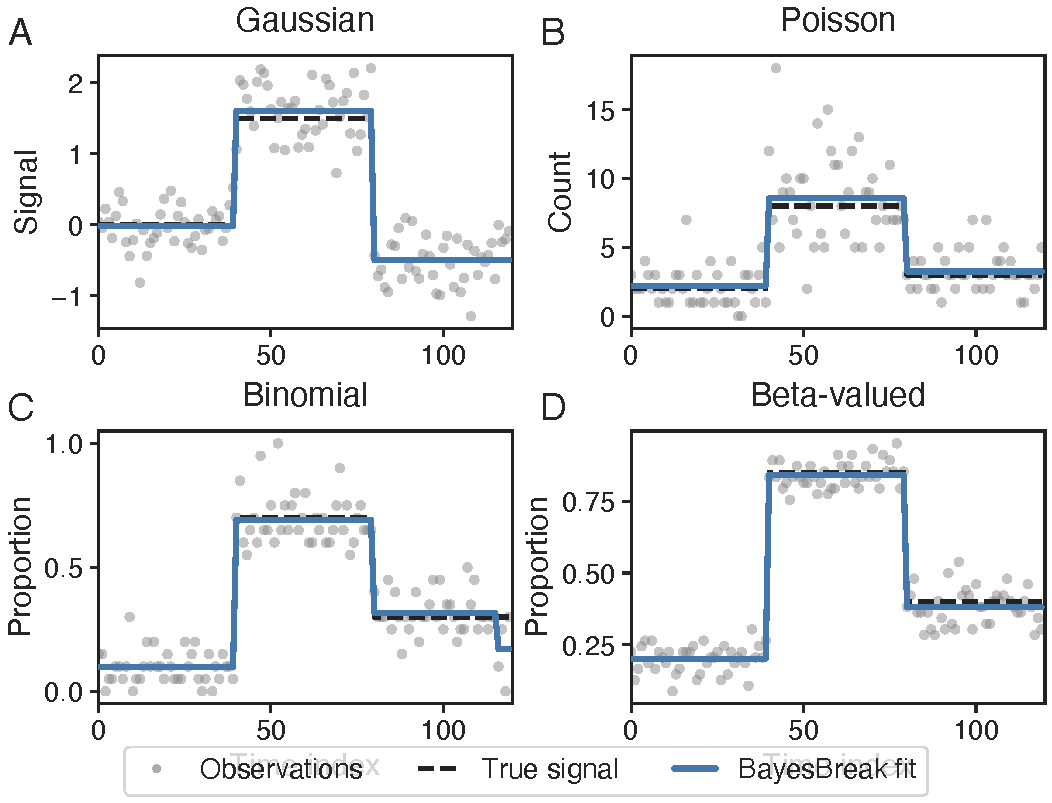
\includegraphics[width=\textwidth]{shared/figures/results/fig2_family_showcase.pdf}
    \caption{Likelihood-family showcase. The first three panels use closed-form conjugate block integrals (Gaussian, Poisson, and Binomial), while the final panel uses the one-dimensional Beta-response quadrature routine. In each case the fitted BayesBreak signal is close to the true piecewise-constant latent parameter.}
    \label{fig:family_showcase}
\end{figure}

\subsection{Quantitative summary across families}

Table~\ref{tab:single_quant} aggregates the small synthetic benchmark packaged with the archive.
The main takeaway is not that one family universally dominates another, but that the same DP
backend remains usable across very different block models. The Poisson setting is visibly the most
challenging among the archived examples: it exhibits the weakest boundary F1 and the largest
reconstruction error, which is consistent with the higher count variability shown in
Figure~\ref{fig:family_showcase}. By contrast, the Beta-response quadrature example achieves the
strongest boundary recovery in this small benchmark.

\begin{table}[H]
    \centering
    \begin{tabular}{lrrrrrrr}\toprule
Family & n & $k^\star$ & $\hat{k}$ & F1@$\tau$ & MAE & MSE & $-\log p(y)/n$\\\midrule
Gaussian & 120 & 3 & 3 & 0.968 & 0.00 & 0.0023 & 0.191\\
Poisson & 120 & 3 & 4 & 0.777 & 0.20 & 0.4501 & 2.162\\
Binomial & 120 & 3 & 3 & 0.960 & 0.06 & 0.0004 & 2.108\\
Beta-valued & 120 & 3 & 3 & 1.000 & 0.00 & 0.0001 & 2.620\\
\bottomrule\end{tabular}

    \caption{Available synthetic summary across the bundled family-specific examples. The final row corresponds to the Beta-response quadrature example rather than to a conjugate closed-form model.}
    \label{tab:single_quant}
\end{table}

Because the table reflects one archived benchmark configuration rather than a large Monte Carlo
study, the numbers serve as a compact portability and relative-difficulty summary, not as
a definitive cross-family ranking.

\subsection{Calibration of boundary posterior probabilities}

A central advantage of the Bayesian formulation is that it returns marginal posterior probabilities
for boundary events. Figure~\ref{fig:calibration} checks whether those probabilities are
calibrated under repeated Gaussian simulations. The reliability curve tracks the diagonal closely
across the full probability range, with an empirical calibration error reported in the figure
inset of approximately $\mathrm{ECE}\approx 0.010$ and Brier score $\approx 0.011$. The
mid-probability bins remain the noisiest because boundary events are intrinsically rare per
sequence, but the ordering of confidence levels is sensible: bins assigned larger posterior
boundary probability correspond to larger empirical boundary frequency.

\begin{figure}[H]
    \centering
    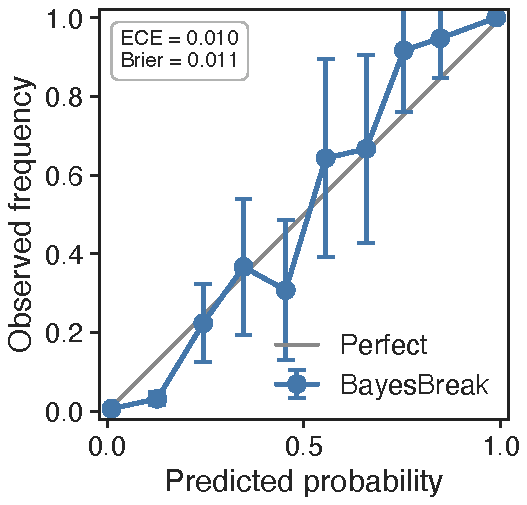
\includegraphics[width=0.78\textwidth]{shared/figures/results/fig3_boundary_calibration.pdf}
    \caption{Calibration of marginal boundary posterior probabilities under synthetic Gaussian data. The dashed diagonal denotes perfect calibration; the orange curve is the empirical frequency within bins of predicted probability.}
    \label{fig:calibration}
\end{figure}

This experiment is valuable because segmentation methods are often judged only by recovered
changepoints. For BayesBreak, well-behaved posterior probabilities are equally important: they
control downstream thresholding, boundary ranking, and any decision rule that is sensitive to the
strength of evidence rather than just to the best segmentation.

\subsection{Latent-group pooling}

Figure~\ref{fig:latent_groups} evaluates the finite latent-group template model on $n_{\mathrm{seq}}=24$
synthetic Gaussian sequences ($n=80$, $\sigma=1.0$) drawn from two groups with different
changepoint patterns. The left panel shows the posterior responsibilities sorted by truth: the
two groups are almost separable, with a small ambiguous band near the class boundary
corresponding to a single mis-assignment (hard accuracy $96\%$). The right panel reports the
group-specific boundary marginals induced by the fitted templates; both groups concentrate their
posterior mass at the correct latent changepoints, with the cluster-1 marginal locating both
boundaries near probability one and the cluster-0 marginal recovering its second boundary at
$t\!\approx\!53$ and a softer mode near $t\!\approx\!26$ for the first.

\begin{figure}[H]
    \centering
    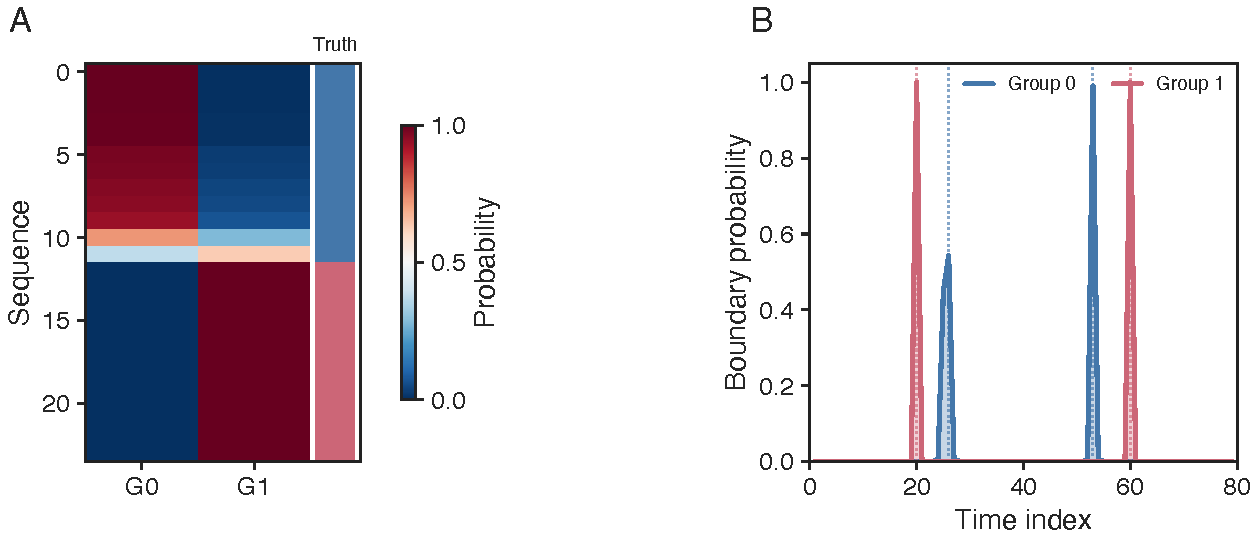
\includegraphics[width=0.82\textwidth]{shared/figures/results/fig4_latent_groups_cropped.pdf}
    \caption{Latent-group pooling on synthetic Gaussian sequences ($n=80$, $\sigma=1.0$, $n_{\mathrm{seq}}=24$). Left: posterior responsibilities $r_{sg}$ for each sequence and score-template group, sorted by truth; the right-hand stripe encodes the true label. Right: group-specific marginal boundary probabilities under the fitted latent templates, with dotted vertical lines marking the true per-group changepoints.}
    \label{fig:latent_groups}
\end{figure}

A six-panel companion diagnostic (uncropped figure \path{shared/figures/results/fig4_latent_groups.pdf})
unpacks the same fit further: per-group example sequences with the inferred piecewise mean,
the boundary marginals, the responsibility heatmap, the group-averaged signal, and a
per-sequence assignment-confidence diagnostic that plots $r_{s,y_s}$ (responsibility on the
true group) sorted along the $x$-axis, with the $0.5$ decision threshold shaded and any
mis-assigned sequences circled. Even when overall accuracy is high, this view exposes which
sequences sit close to the decision boundary and is informative regardless of whether any
hard mistakes are made.

\subsection{Non-conjugate approximation trade-offs}

For non-conjugate likelihoods, BayesBreak relies on approximate block evidences while reusing the
same DP layer. Table~\ref{tab:nonconj_tradeoff} compares several such approximations in a bundled
logistic-normal synthetic example, using numerical quadrature as a reference. The table shows the
observed speed--accuracy trade-off in this archived example: Laplace is the fastest among the listed approximations, while exact quadrature is the slowest. At the same time, block-level approximation error
is not perfectly monotone with segmentation quality, because the DP aggregates many local scores
nonlinearly.

\begin{table}[H]
    \centering
    \begin{tabular}{lrrrrrr}\toprule
Method & $\max|\Delta \log A^0|$ & $q_{95}|\Delta \log A^0|$ & median $|\Delta \log A^0|$ & time (s) & F1@$\tau$ & $\hat{k}$\\\midrule
quadrature & 0.000 & 0.000 & 0.000 & 0.093 & 0.286 & 6\\
laplace & 1.235 & 1.188 & 0.980 & 0.049 & 0.286 & 6\\
jj & 1.265 & 1.216 & 1.002 & 0.071 & 0.500 & 3\\
ep & 14.502 & 14.141 & 12.680 & 0.059 & 0.500 & 7\\
pg-vb & 1.265 & 1.216 & 1.002 & 0.072 & 0.500 & 3\\
\bottomrule\end{tabular}

    \caption{Approximation trade-offs for a non-conjugate Bernoulli/logistic block model. Quadrature is used as the local reference block integral; the remaining methods trade block-level fidelity against computational cost.}
    \label{tab:nonconj_tradeoff}
\end{table}

\paragraph{Connection to Proposition~\ref{prop:stability}.}
The large reported values of $\max|\Delta\log A|$ in Table~\ref{tab:nonconj_tradeoff} (several to
tens of log units on the worst reachable block for some approximations) place this illustration outside the small-$\varepsilon$ regime where the uniform-error
bound in Proposition~\ref{prop:stability} is tight.
The boundary F1 values are therefore descriptive diagnostics, not a confirmation of the
small-$\varepsilon$ regime. The table still usefully shows that block-level error, runtime, and
segmentation quality need not move monotonically together, but it is not a universal ranking of
non-conjugate approximation methods.

\subsection{Runtime scaling}

Finally, Figure~\ref{fig:runtime} and Table~\ref{tab:runtime_scaling} report runtime behavior for
the Gaussian implementation. Panel~A sweeps the series length $n\in\{50,100,200,400,800\}$ at two
fixed segment budgets $k_{\max}\in\{10,20\}$; panel~B sweeps the segment budget
$k_{\max}\in\{5,10,20,40,80\}$ at fixed $n=200$. Over the archived range, the empirical log-log
slopes annotated on Figure~\ref{fig:runtime} are $\approx 1.07$ in $n$ at $k_{\max}=10$,
$\approx 1.14$ in $n$ at $k_{\max}=20$, and $\approx 0.88$ in $k_{\max}$ at fixed $n=200$. Both
sweeps therefore sit well below the $\mathcal{O}(k_{\max}n^2)$ worst case predicted by the exact
sum-product DP. The discrepancy reflects two practical effects: (i) cumulative
sufficient-statistics caching makes each candidate block evaluation effectively constant time, so
the DP cost reduces to traversing the $\mathcal{O}(k_{\max}n)$ reachable $(k,\text{end-point})$
pairs over the small archived range; and (ii) constant-factor overhead from prior evaluation and
DP setup dominates at the smallest $n$, flattening the small-$n$ end of the curve. The
$\mathcal{O}(k_{\max}n^2)$ worst case still controls the asymptotic profile and is the relevant
bound for the much larger $n$ regimes flagged for the next-pass scaling study in
Remark~\ref{rem:mem-time}.

\begin{figure}[H]
    \centering
    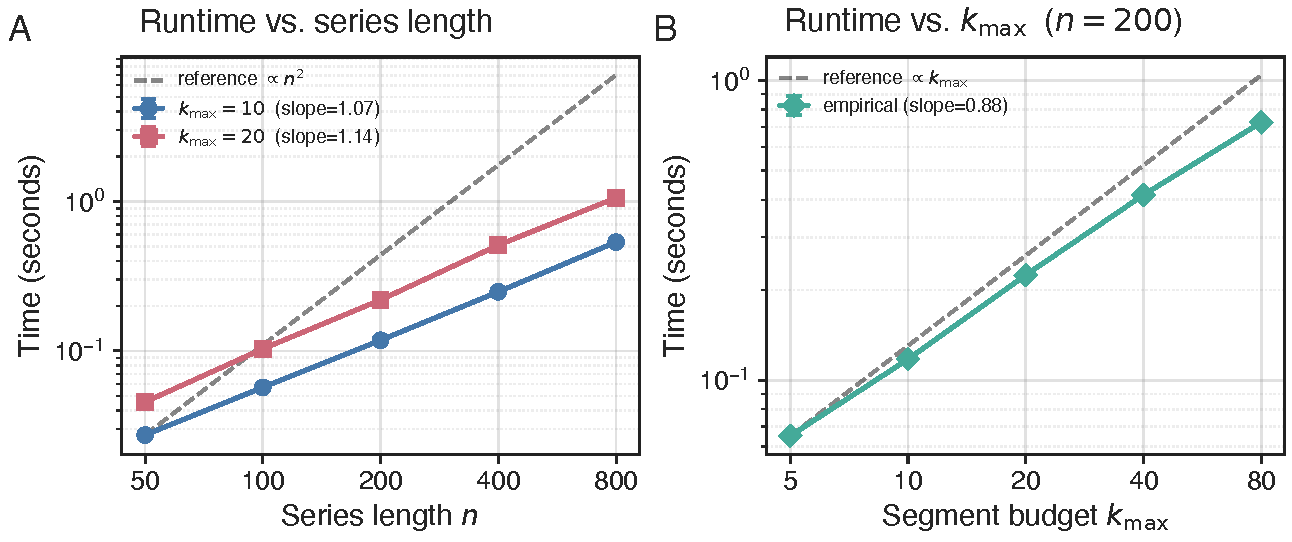
\includegraphics[width=\textwidth]{shared/figures/results/fig5_runtime_scaling.pdf}
    \caption{Runtime scaling for the Gaussian implementation. Panel A: log-log wall-clock time vs.\ series length $n\in\{50,100,200,400,800\}$ at two segment budgets $k_{\max}\in\{10,20\}$; annotated slopes give the empirical $\log t$ vs.\ $\log n$ exponent for each curve, and a dashed reference line shows the theoretical $\mathcal{O}(n^2)$ worst case anchored at the smallest measured point. Panel B: log-log time vs.\ $k_{\max}\in\{5,10,20,40,80\}$ at fixed $n=200$ with a dashed linear-in-$k_{\max}$ reference. Points are means over 5 repetitions; error bars denote one standard deviation.}
    \label{fig:runtime}
\end{figure}

\begin{table}[H]
    \centering
    \begin{tabular}{rrrr}\toprule
n & $k_{\max}$ & mean (s) & std (s)\\\midrule
50 & 20 & 0.0455 & 0.0008\\
100 & 20 & 0.1033 & 0.0011\\
200 & 20 & 0.2195 & 0.0011\\
400 & 20 & 0.5106 & 0.0307\\
800 & 20 & 1.0585 & 0.0345\\
\bottomrule\end{tabular}

    \caption{Numerical companion for the same archived Gaussian runtime configuration as Figure~\ref{fig:runtime}. The bundled table reports the $k_{\max}=20$ configuration of panel~A rather than every curve displayed in the figure; the $k_{\max}$ sweep of panel~B is recorded in the figure's CSV sidecar.}
    \label{tab:runtime_scaling}
\end{table}


\section{Evidence interpretation}
All populated values and panels in this chapter are real archived computations. Their role is
method validation on the bundled synthetic settings, not a comprehensive state-of-the-art claim.
Boundary calibration reports ECE approximately $0.010$ and Brier approximately $0.011$. The
latent-group template experiment reports 96\% hard recovery at $\sigma=1.0$ for 24 sequences.
The runtime fits report log--log slopes about $1.07$ at $k_{\max}=10$ and $1.14$ at
$k_{\max}=20$ for $n=50,\ldots,800$; these are local empirical summaries, not an asymptotic
complexity result.

\begin{figure}[H]
\centering
\resizebox{0.96\textwidth}{!}{\begin{tikzpicture}[node distance=7mm and 8mm]
\node[primarybox,text width=23mm] (claim) {Statistical claim};
\node[secondarybox,right=of claim,text width=28mm] (hyp) {Hypothesis and competing explanation};
\node[primarybox,right=of hyp,text width=25mm] (protocol) {Data-generating process or dataset, estimand, and metric};
\node[primarybox,right=of protocol,text width=24mm] (run) {Executed calculation and recorded output};
\node[successbox,right=of run,text width=27mm] (decision) {Permitted scientific interpretation};
\draw[arrPrimary] (claim)--(hyp);
\draw[arrPrimary] (hyp)--(protocol);
\draw[arrPrimary] (protocol)--(run);
\draw[arrPrimary] (run)--(decision);
\node[draw=Warning,fill=WarningPale,rounded corners,below=9mm of run,text width=32mm,align=center] (excluded) {Exclude when the observation model, coordinate axis, reference, or metric is incompatible};
\draw[arr,draw=Warning] (run)--(excluded);
\end{tikzpicture}
}
\caption{Relation among claims, experiments, and interpretation. An executed computation is excluded from a stated conclusion when its observation model, coordinate axis, reference quantity, or metric is incompatible with that conclusion.}
\label{fig:claim-experiment-map}
\end{figure}

\section{Coverage still required}
The archive does not yet provide full repeated uncertainty intervals, fairness-controlled external
comparators across every family, large-$n$ scaling, or complete misspecification grids. These are
specified as protocols in Appendix~\ref{app:experiments}; no planned cell is populated in this
chapter.
